\documentclass[tikz]{standalone}

\definecolor{myred}{RGB}{196,19,47}
 
\usetikzlibrary{decorations.pathreplacing}


\makeatletter
\tikzset{manifold/.style={
  to path={
    \pgfextra{
    \def\tikz@to@out{20}\tikz@to@switch@on
    }
    (\tikztostart) -- (\tikztostart -| \tikztotarget)
    -- (\tikztotarget)
    -- (\tikztostart |- \tikztotarget)
    -- cycle
    (\tikztotarget)
    \tikztonodes
  }
}}
\makeatother

\begin{document}

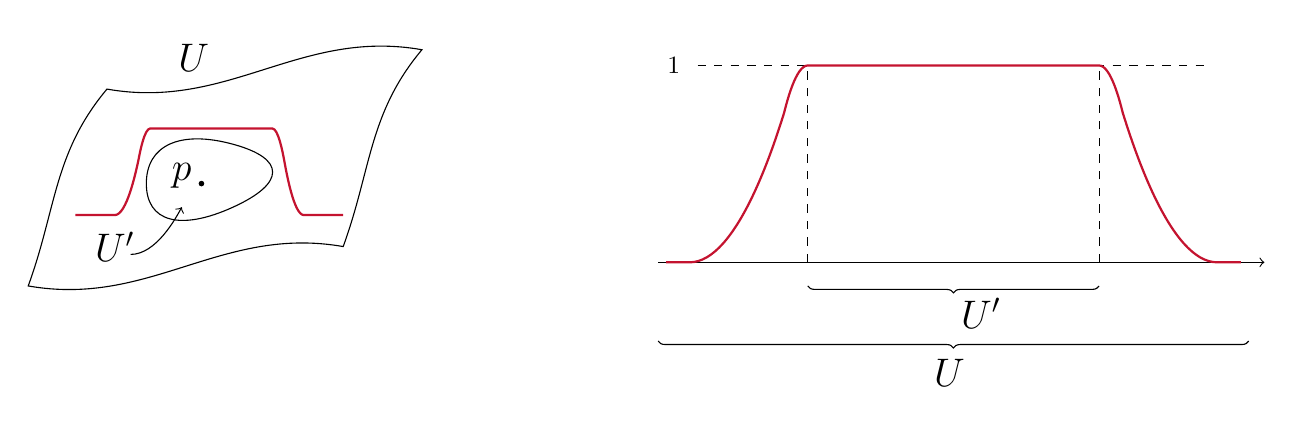
\begin{tikzpicture}


  % base manifold
  \draw[thin] (0,0)
   to[out=-10,in=170] (4,0.5)
    to[out=70,in=-130] (5,3) 
    to[out=170,in=-10] (1,2.5) 
    to[out=-130,in=70] cycle;

  % manifold inside with text etc.
  \begin{scope}[shift={(-0.4,-0.2)},out=-20,in=160,relative]
       \node (p1) at (1.9, 1.5) {};
   \node (p2) at (3, 1.2) {};
   \node (p3) at (3, 2) {};
    \path[draw, black]plot [smooth cycle,tension=2.2] coordinates {(p1) (p2) (p3)};
    \filldraw (2.6,1.5)circle (0.8pt);
    \node at (2.35,1.6) {\Large$p$};
    \node at (1.5,0.7) {\Large$U'$};
    \draw[->] (1.7,0.6) parabola  (2.35,1.2);
    \node at (2.5,3.1) {\Large$U$};

    
  \end{scope}
  
    % bump function inside
   \begin{scope}
     \draw[thick,color=myred] (0.6,0.9) to (1.1,0.9)
     parabola[bend at start] (1.4,1.6)
     parabola[bend at end] (1.55,2)
     to (3.1,2)
     parabola[bend at start] (3.25,1.6)
     parabola[bend at end] (3.5,0.9)
	 to (4,0.9);
   \end{scope}


  % right side
  \begin{scope}[shift={(8.5,0)}]
    \draw[dashed, thin] (0,2.8) -- (6.5,2.8);
    \node at (-0.3,2.8) {\small$1$};
    \draw[thin, ->] (-0.5,0.3) -- (7.2,0.3);
    
    \draw[thick,color=myred] (-0.4,0.3)
    to (-0.1,0.3)
    parabola[bend at start] (1.1,2.2)
    parabola[bend at end](1.4,2.8) 
    parabola[bend at end](1.9,2.8)
    to (4.6,2.8)
    parabola[bend at start] (5.1,2.8)
    parabola[bend at start] (5.4,2.2)
    parabola[bend at end](6.6,0.3)
    to (6.9,0.3);
    
	% dashed lines
	\draw[thin,dashed] (1.4,0.3) to (1.4,2.8);
	\draw[thin,dashed] (5.1,0.3) to (5.1,2.8);
  \end{scope}
  
  % underbraces
   \begin{scope}[shift={(8.5,0)}]
     \draw [thin, decoration={brace,mirror,raise=0.5cm},decorate] (1.4,0.5) -- (5.1,0.5);
     \node at (3.6,-0.35) {\Large$U'$};
     \draw [thin, decoration={brace,mirror,raise=0.5cm},decorate] (-0.5,-0.2) -- (7,-0.2);
     \node at (3.2,-1.1) {\Large$U$};
   \end{scope}
\end{tikzpicture}
\end{document}